\documentclass[11pt,letterpaper]{scrartcl}
\usepackage{graphicx}
\usepackage{booktabs}
\usepackage{verbatim}

\begin{document}
\titlehead{\centering Guam Coconut Rhinoceros Beetle Biocontrol Project Technical Report}
\title{OrNV Transmission Experiment}
\author{James Grasela and Aubrey Moore}
\maketitle

\begin{abstract}
	This experiment was performed to determine if OrNV isolate V23B can be transmitted from a dosed CRB adult to an undosed CRB 
	adult.
\end{abstract}

\begin{scriptsize}
\begin{verbatim}
@misc{grasela_guam_2020,
  title = {Guam {{CRB Biocontrol Project Technical Report}}: {{OrNV Transmission Experiment}}},
  author = {Grasela, James and Moore, Aubrey},
  date = {2020},
  url = {https://github.com/aubreymoore/OrNV-Transmission/blob/master/ornv-transmission.pdf}
}
\end{verbatim}
\end{scriptsize}

\newpage

\section{Materials and Methods}

\subsection{Beetles}

Beetles were field collected from pheromone sites and kept individually in moist peat moss in Mason jars. The jars were held under 
standard rearing conditions in an environmental chamber: 30 deg C; 80\% RH; 12h photoperiod.

\subsection{Virus and Dosing Method}

Beetles were dosed per os with ca. 30 microlitre V23B virus preparation of unknown concentration (AgResearch, New Zealand).

\subsection{Experimental design}

To test for virus transmission, beetles were selected at random and assigned to 45 pairs with a male and a female 
in each pair. These pairs were housed in Mason jars half filled with moist peat moss. The jars were held under 
standard rearing conditions. At the start of the bioassay, the beetle pairs were randomly placed in 3 treatment groups of 15 jars each. Beetles were observed every other day.

\subsection{Post-mortems}

Dead beetles were dissected and images were made of guts using a cellphone camera. Note on pathology were recorded.


\section{Analysis}

Data were saved in a comma separated values text file, \textbf{OrNV-transmission.csv}. Analysis was performed using a Jupyter notebook, \textbf{OrNV-transmission.ipynb}.

\begin{table}[h]
	\centering
\caption{Treatment groups.}
	
\begin{tabular}{ll}
	\toprule
	Treatment group & Treatment\\
	\midrule
	Jars labeled C1 through C15 & Experimental control; neither beetle was dosed\\
    Jars labeled TF1 through TF15 & Female was dosed with virus; male was not dosed\\
    Jars labeled MF1 through MF15 & Female was dosed with virus; male was not dosed\\
	\bottomrule
\end{tabular} 

\end{table}

\section{Results}

Results from this experiment are inconclusive because ofh high control mortality (Fig. \ref{fig:survivorship}).

\begin{figure}[h]
\centering
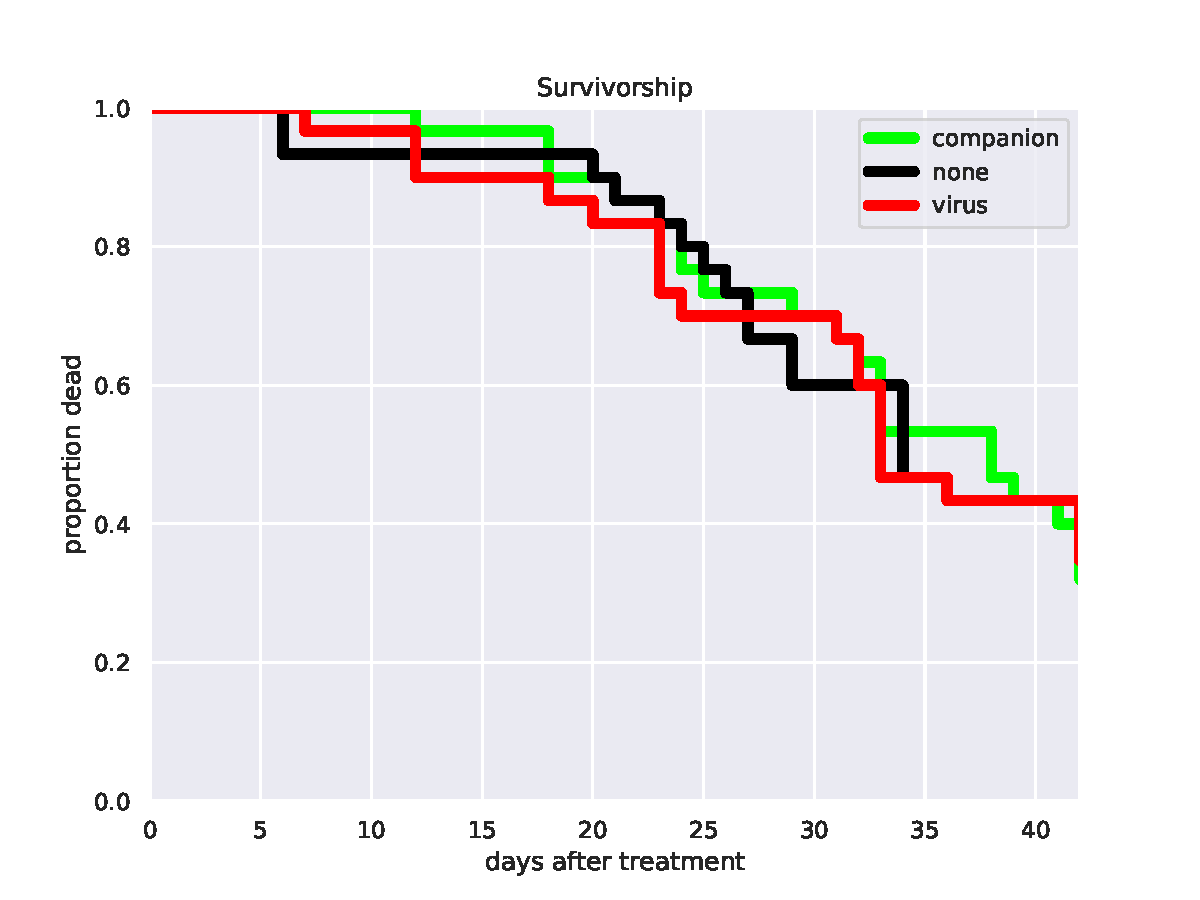
\includegraphics[width=\textwidth]{survivorship.pdf}
\caption{Survival of beetles after treatment.}
\label{fig:survivorship}
\end{figure}

\begin{figure}[h]
\centering
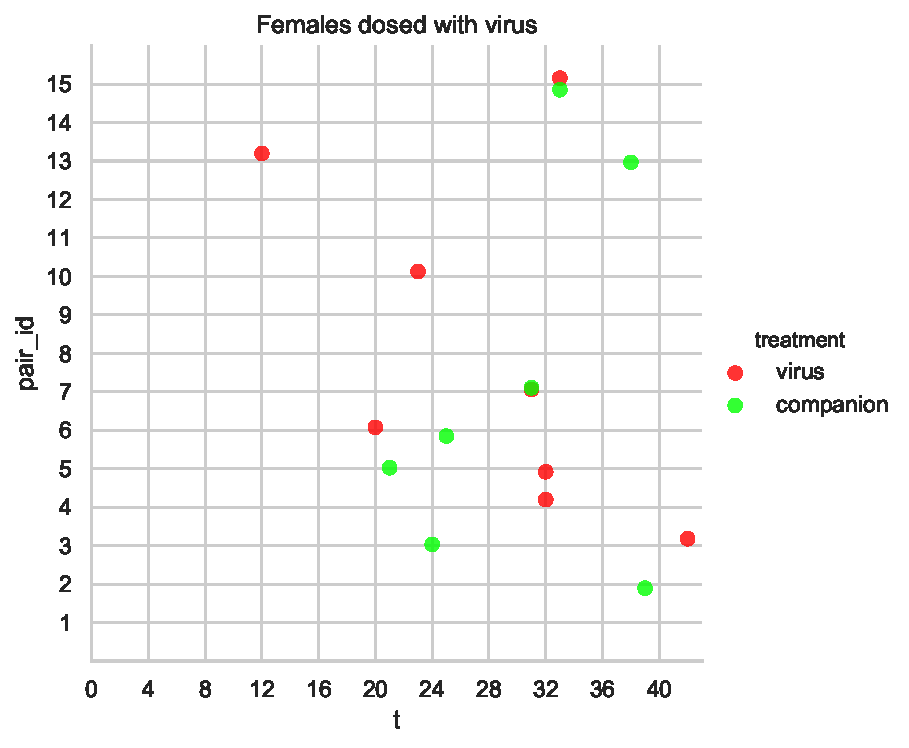
\includegraphics[width=\textwidth]{tf.pdf}
\caption{Mortality of beetles in jars where the female was dosed with virus. Points indicate time of death, in days after treatment, for dosed (red points) and undosed beetles (green points).}
\label{fig:tf}
\end{figure}

\begin{figure}[h]
\centering
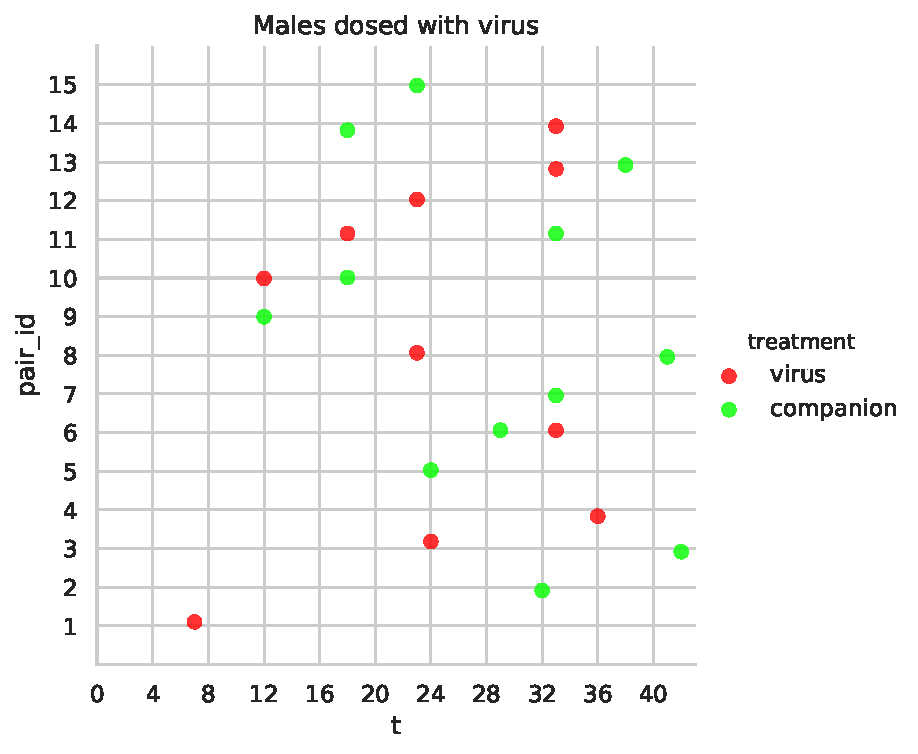
\includegraphics[width=\textwidth]{tm.pdf}
\caption{Mortality of beetles in jars where the male was dosed with virus. Points indicate time of death, in days after treatment, for dosed (red points) and undosed beetles (green points).}
\label{fig:tm}
\end{figure}

\clearpage
\appendix

\section{Data file: ornv-transmission-1.csv}

\begin{tiny}
\verbatiminput{ornv-transmission-1.csv}
\end{tiny}

\clearpage

\section{Post-mortem images}


\begin{figure}[]
\centering
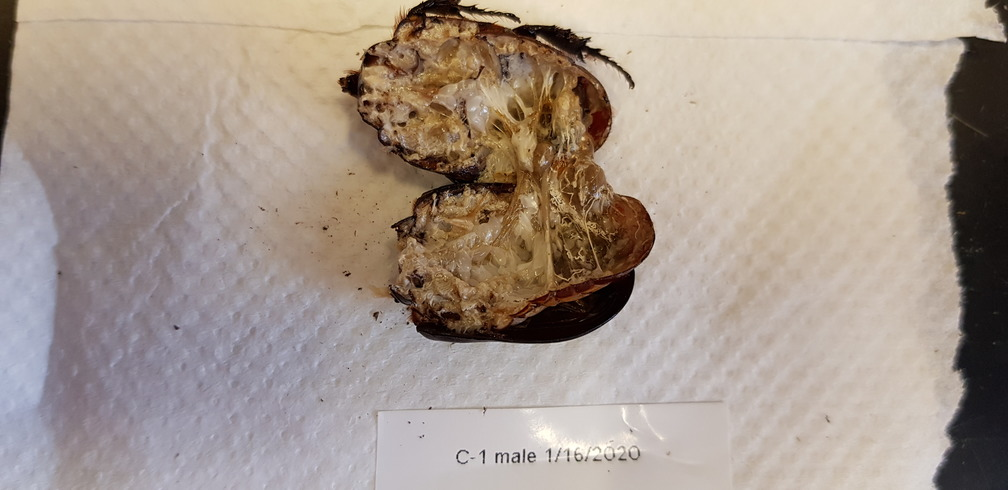
\includegraphics[width=\textwidth]{pm-images/20200116_110145_001.jpg}
\caption{Caption}
\end{figure}

        \clearpage
        
\begin{figure}[]
\centering
\includegraphics[width=\textwidth]{pm-images/20200129_145244.jpg}
\caption{Caption}
\end{figure}

        \clearpage
        
\begin{figure}[]
\centering
\includegraphics[width=\textwidth]{pm-images/20200119_121343.jpg}
\caption{Caption}
\end{figure}

        \clearpage
        
\begin{figure}[]
\centering
\includegraphics[width=\textwidth]{pm-images/20200121_112302.jpg}
\caption{Caption}
\end{figure}

        \clearpage
        
\begin{figure}[]
\centering
\includegraphics[width=\textwidth]{pm-images/20200210_150730.jpg}
\caption{Caption}
\end{figure}

        \clearpage
        
\begin{figure}[]
\centering
\includegraphics[width=\textwidth]{pm-images/20200102_112827.jpg}
\caption{Caption}
\end{figure}

        \clearpage
        
\begin{figure}[]
\centering
\includegraphics[width=\textwidth]{pm-images/20200123_163747.jpg}
\caption{Caption}
\end{figure}

        \clearpage
        
\begin{figure}[]
\centering
\includegraphics[width=\textwidth]{pm-images/20200125_122409.jpg}
\caption{Caption}
\end{figure}

        \clearpage
        
\begin{figure}[]
\centering
\includegraphics[width=\textwidth]{pm-images/20200211_095032.jpg}
\caption{Caption}
\end{figure}

        \clearpage
        
\begin{figure}[]
\centering
\includegraphics[width=\textwidth]{pm-images/20200210_151921.jpg}
\caption{Caption}
\end{figure}

\begin{figure}[]
\centering
\includegraphics[width=\textwidth]{pm-images/20200129_151721.jpg}
\caption{Caption}
\end{figure}

        \clearpage
        
\begin{figure}[]
\centering
\includegraphics[width=\textwidth]{pm-images/20200210_145205.jpg}
\caption{Caption}
\end{figure}

        \clearpage
        
\begin{figure}[]
\centering
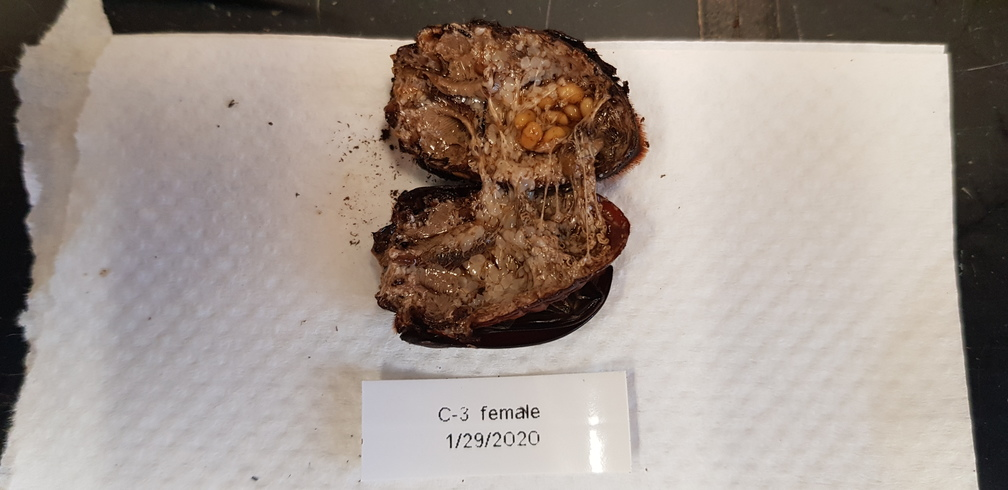
\includegraphics[width=\textwidth]{pm-images/20200129_161111.jpg}
\caption{Caption}
\end{figure}

        \clearpage
        
\begin{figure}[]
\centering
\includegraphics[width=\textwidth]{pm-images/20200131_113359.jpg}
\caption{Caption}
\end{figure}

        \clearpage
        
\begin{figure}[]
\centering
\includegraphics[width=\textwidth]{pm-images/20200129_143353.jpg}
\caption{Caption}
\end{figure}

        \clearpage
        
\begin{figure}[]
\centering
\includegraphics[width=\textwidth]{pm-images/20200116_110642.jpg}
\caption{Caption}
\end{figure}

        \clearpage
        
\begin{figure}[]
\centering
\includegraphics[width=\textwidth]{pm-images/20200102_112130.jpg}
\caption{Caption}
\end{figure}

        \clearpage
        
\begin{figure}[]
\centering
\includegraphics[width=\textwidth]{pm-images/20200123_163225.jpg}
\caption{Caption}
\end{figure}

        \clearpage
        
\begin{figure}[]
\centering
\includegraphics[width=\textwidth]{pm-images/20200125_121834.jpg}
\caption{Caption}
\end{figure}

        \clearpage
        
\begin{figure}[]
\centering
\includegraphics[width=\textwidth]{pm-images/20200119_121825.jpg}
\caption{Caption}
\end{figure}

\begin{figure}[]
\centering
\includegraphics[width=\textwidth]{pm-images/20200210_151339.jpg}
\caption{Caption}
\end{figure}

        \clearpage
        
\begin{figure}[]
\centering
\includegraphics[width=\textwidth]{pm-images/20200121_113027.jpg}
\caption{Caption}
\end{figure}

        \clearpage
        
\begin{figure}[]
\centering
\includegraphics[width=\textwidth]{pm-images/20200210_152419.jpg}
\caption{Caption}
\end{figure}

        \clearpage
        
\begin{figure}[]
\centering
\includegraphics[width=\textwidth]{pm-images/20200210_145811.jpg}
\caption{Caption}
\end{figure}

        \clearpage
        
\begin{figure}[]
\centering
\includegraphics[width=\textwidth]{pm-images/20200203_114327.jpg}
\caption{Caption}
\end{figure}

        \clearpage
        
\begin{figure}[]
\centering
\includegraphics[width=\textwidth]{pm-images/20200114_104530.jpg}
\caption{Caption}
\end{figure}

        \clearpage
        
\begin{figure}[]
\centering
\includegraphics[width=\textwidth]{pm-images/20200116_111311.jpg}
\caption{Caption}
\end{figure}

        \clearpage
        
\begin{figure}[]
\centering
\includegraphics[width=\textwidth]{pm-images/20200121_111727.jpg}
\caption{Caption}
\end{figure}

        \clearpage
        
\begin{figure}[]
\centering
\includegraphics[width=\textwidth]{pm-images/20191229_120148.jpg}
\caption{Caption}
\end{figure}

        \clearpage
        
\begin{figure}[]
\centering
\includegraphics[width=\textwidth]{pm-images/20200129_153950.jpg}
\caption{Caption}
\end{figure}

\begin{figure}[]
\centering
\includegraphics[width=\textwidth]{pm-images/20200127_151015.jpg}
\caption{Caption}
\end{figure}

        \clearpage
        
\begin{figure}[]
\centering
\includegraphics[width=\textwidth]{pm-images/20200206_113817.jpg}
\caption{Caption}
\end{figure}

        \clearpage
        
\begin{figure}[]
\centering
\includegraphics[width=\textwidth]{pm-images/20200127_145553.jpg}
\caption{Caption}
\end{figure}

        \clearpage
        
\begin{figure}[]
\centering
\includegraphics[width=\textwidth]{pm-images/20200116_112000.jpg}
\caption{Caption}
\end{figure}

        \clearpage
        
\begin{figure}[]
\centering
\includegraphics[width=\textwidth]{pm-images/20200127_144326.jpg}
\caption{Caption}
\end{figure}

        \clearpage
        
\begin{figure}[]
\centering
\includegraphics[width=\textwidth]{pm-images/20200119_123529.jpg}
\caption{Caption}
\end{figure}

        \clearpage
        
\begin{figure}[]
\centering
\includegraphics[width=\textwidth]{pm-images/20200108_101434.jpg}
\caption{Caption}
\end{figure}

        \clearpage
        
\begin{figure}[]
\centering
\includegraphics[width=\textwidth]{pm-images/20200129_153605.jpg}
\caption{Caption}
\end{figure}

        \clearpage
        
\begin{figure}[]
\centering
\includegraphics[width=\textwidth]{pm-images/20200102_111008.jpg}
\caption{Caption}
\end{figure}

        \clearpage
        
\begin{figure}[]
\centering
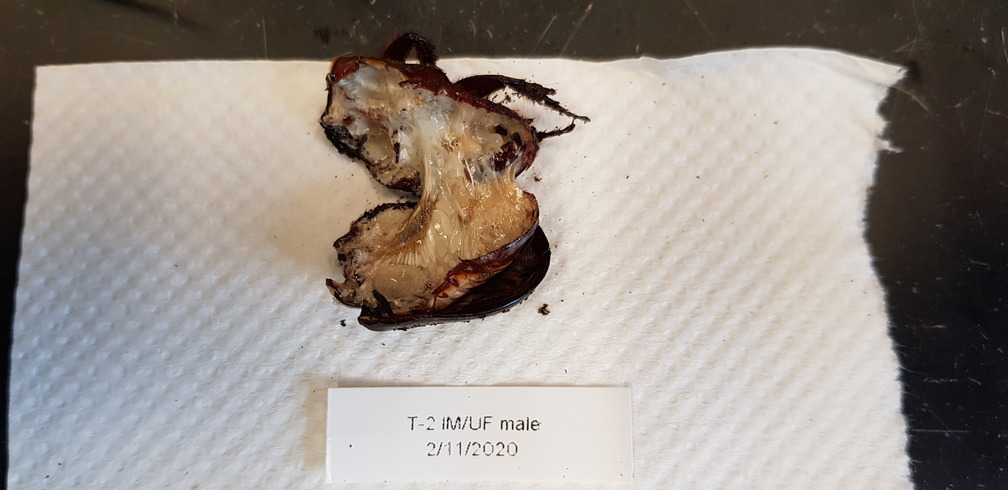
\includegraphics[width=\textwidth]{pm-images/20200211_114845_001.jpg}
\caption{Caption}
\end{figure}

\begin{figure}[]
\centering
\includegraphics[width=\textwidth]{pm-images/20200119_122916.jpg}
\caption{Caption}
\end{figure}

        \clearpage
        
\begin{figure}[]
\centering
\includegraphics[width=\textwidth]{pm-images/20200131_115718.jpg}
\caption{Caption}
\end{figure}

        \clearpage
        
\begin{figure}[]
\centering
\includegraphics[width=\textwidth]{pm-images/20200119_115644.jpg}
\caption{Caption}
\end{figure}

        \clearpage
        
\begin{figure}[]
\centering
\includegraphics[width=\textwidth]{pm-images/20200108_102337.jpg}
\caption{Caption}
\end{figure}

        \clearpage
        
\begin{figure}[]
\centering
\includegraphics[width=\textwidth]{pm-images/20200114_105113.jpg}
\caption{Caption}
\end{figure}

        \clearpage
        
\begin{figure}[]
\centering
\includegraphics[width=\textwidth]{pm-images/20200119_122428.jpg}
\caption{Caption}
\end{figure}

        \clearpage
        
\begin{figure}[]
\centering
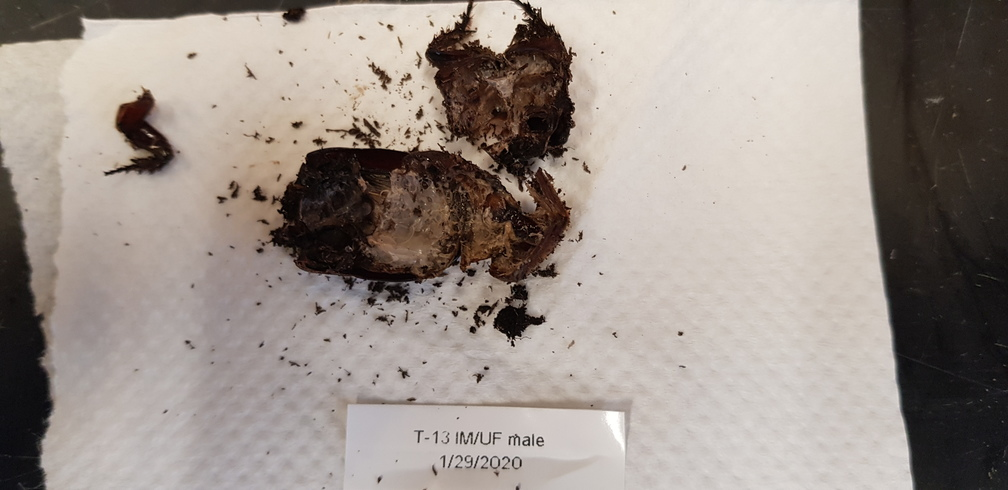
\includegraphics[width=\textwidth]{pm-images/20200129_152333.jpg}
\caption{Caption}
\end{figure}

        \clearpage
        
\begin{figure}[]
\centering
\includegraphics[width=\textwidth]{pm-images/20200129_154608.jpg}
\caption{Caption}
\end{figure}

        \clearpage
        
\begin{figure}[]
\centering
\includegraphics[width=\textwidth]{pm-images/20200127_150141.jpg}
\caption{Caption}
\end{figure}

        \clearpage
        
\begin{figure}[]
\centering
\includegraphics[width=\textwidth]{pm-images/20200206_113320.jpg}
\caption{Caption}
\end{figure}

\begin{figure}[]
\centering
\includegraphics[width=\textwidth]{pm-images/20200119_124629.jpg}
\caption{Caption}
\end{figure}

        \clearpage
        
\begin{figure}[]
\centering
\includegraphics[width=\textwidth]{pm-images/20200108_103227.jpg}
\caption{Caption}
\end{figure}

        \clearpage
        
\begin{figure}[]
\centering
\includegraphics[width=\textwidth]{pm-images/20200114_105656.jpg}
\caption{Caption}
\end{figure}

        \clearpage
        
\begin{figure}[]
\centering
\includegraphics[width=\textwidth]{pm-images/20200129_152948.jpg}
\caption{Caption}
\end{figure}

        \clearpage
        
\begin{figure}[]
\centering
\includegraphics[width=\textwidth]{pm-images/20200203_113806.jpg}
\caption{Caption}
\end{figure}

        \clearpage
        
\begin{figure}[]
\centering
\includegraphics[width=\textwidth]{pm-images/20200114_104047.jpg}
\caption{Caption}
\end{figure}

        \clearpage
        
\begin{figure}[]
\centering
\includegraphics[width=\textwidth]{pm-images/20200119_120121.jpg}
\caption{Caption}
\end{figure}

        \clearpage
        

\clearpage

\end{document}

